\begin{frame}[t]{NPN-Transistor}

  \textbf{Ziel - Darstellung des Ausgangskennlinienfeld}
  
  \begin{spacing}{0.6} \begin{tiny}
  
  Das Ausgangskennlinienfeld eines npn Transistors beschreibt den Zusammenhang von Kollektorstrom $I_c$ und der Spannung 
  an der Kollektor-Emitter Strecke $U_{ce}$. Das Kennlinienfeld wird für verschiedene Basisströme $I_b$ angegeben. 
  \end{tiny} \end{spacing}
  \begin{spacing}{0.9} \begin{tiny}
  \begin{table}[h!]
    \begin{tabular}{p{3cm} p{7cm}}
      \hline
      \textbf{Erstellung des Schaltplans} & \\
      \hline \\
      \begin{minipage}{.3\textwidth}
        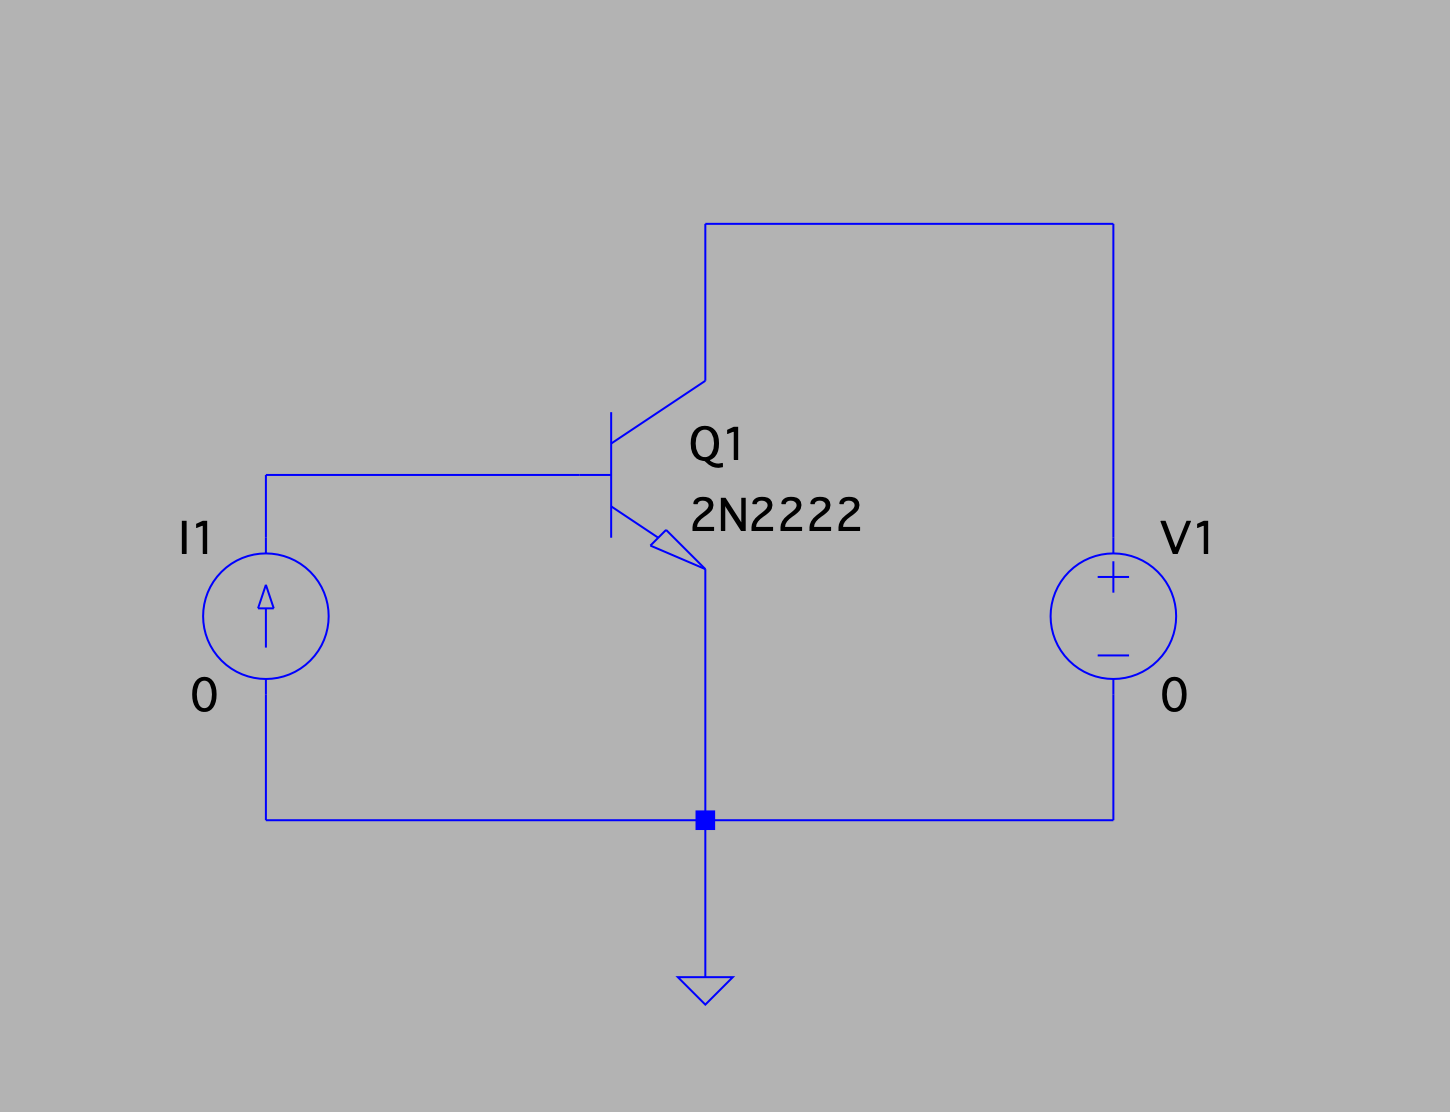
\includegraphics[width=\linewidth]{pictures/tran.png}
      \end{minipage} 
      & 
      \begin{minipage}{.7\textwidth}
      \begin{itemize}
        \item Startet mit einem neuen schematic
        \item Speichert das Projekt direkt als neue Datei ab (File $->$ save as ) 
        \item Fügt eine ideale Stromquelle (\textbf{F2} \dots current) hinzu und dreht dieser (\textbf{STRG+R}) 
        \item Fügt einen npn-Transistor(\textbf{F2} \dots npn) hinzu.
        \item Per rechtem Mausklick könnt ihr vom idealen npn anlaog zur Diode im letzten Beispiel zum 2N2222 wechseln.
        \item Verdrahtet die Schaltung wieder vollstänndig (\textbf{F3})
      \end{itemize}
      \end{minipage} 
      \\
       & \\
       \hline
       \textbf{Konfiguration der Simulation} & \\
       \hline \\
       \begin{minipage}{.3\textwidth}
        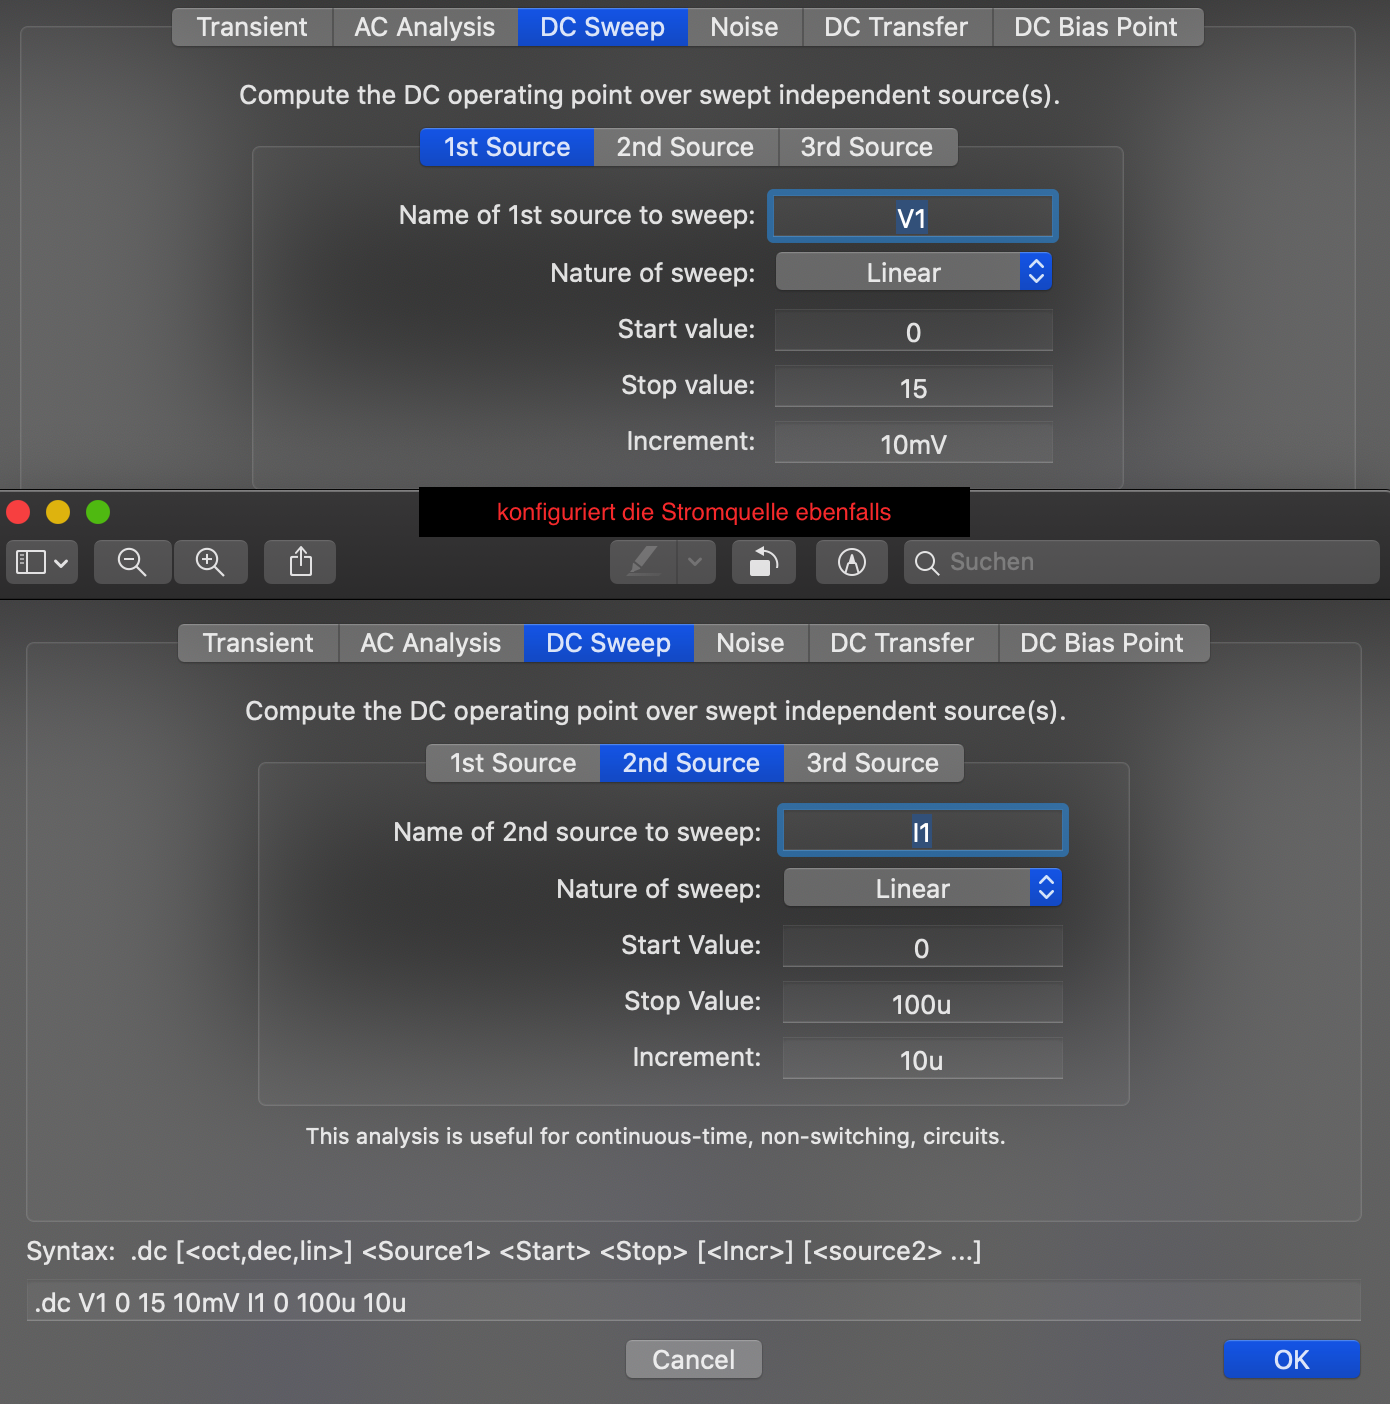
\includegraphics[width=0.8\linewidth]{pictures/simulationcmd_3.png}
      \end{minipage} 
      & 
      \begin{minipage}{.7\textwidth}
      \begin{itemize}
        \item Im Menu Simulation, wählt \textbf{Edit simulation command} und bliebt beim DC Sweep. 
        \item Unser Ziel ist es das Ausgangskennlinienfeld des 2N2222 simlativ zu bestimmen. Dazu verwenden wir einen DC-Sweep 
        mit einer ideal Stromquelle (I1) die verschiedene Basisströme $I_b$ simuliert und eine Spannungsquelle (V1) die die Spannung
        $U_{ce}$ simuliert. 
        \item V1 soll von 0 - 15V in 1V Schritten simuliert werden, I1 von 0 - 100u in 10u Schritten.
        \item Bestätigt mit \textit{OK} und fügt die Simlationsansweisung dem schematic hinzu
      \end{itemize}
      \end{minipage} 
      \\
       & \\
       \hline
    \end{tabular}
  
  \end{table}
  
  \end{tiny} \end{spacing}
  
   \end{frame}
  
   \begin{frame}[t]{NPN-Transistor}
  
    \begin{spacing}{0.9} \begin{tiny}
    \begin{table}[h!]
      \begin{tabular}{p{5cm} p{5cm}}
        \hline
        \textbf{Simulation und Analyse} & \\
        \hline \\
        \begin{minipage}{.5\textwidth}
          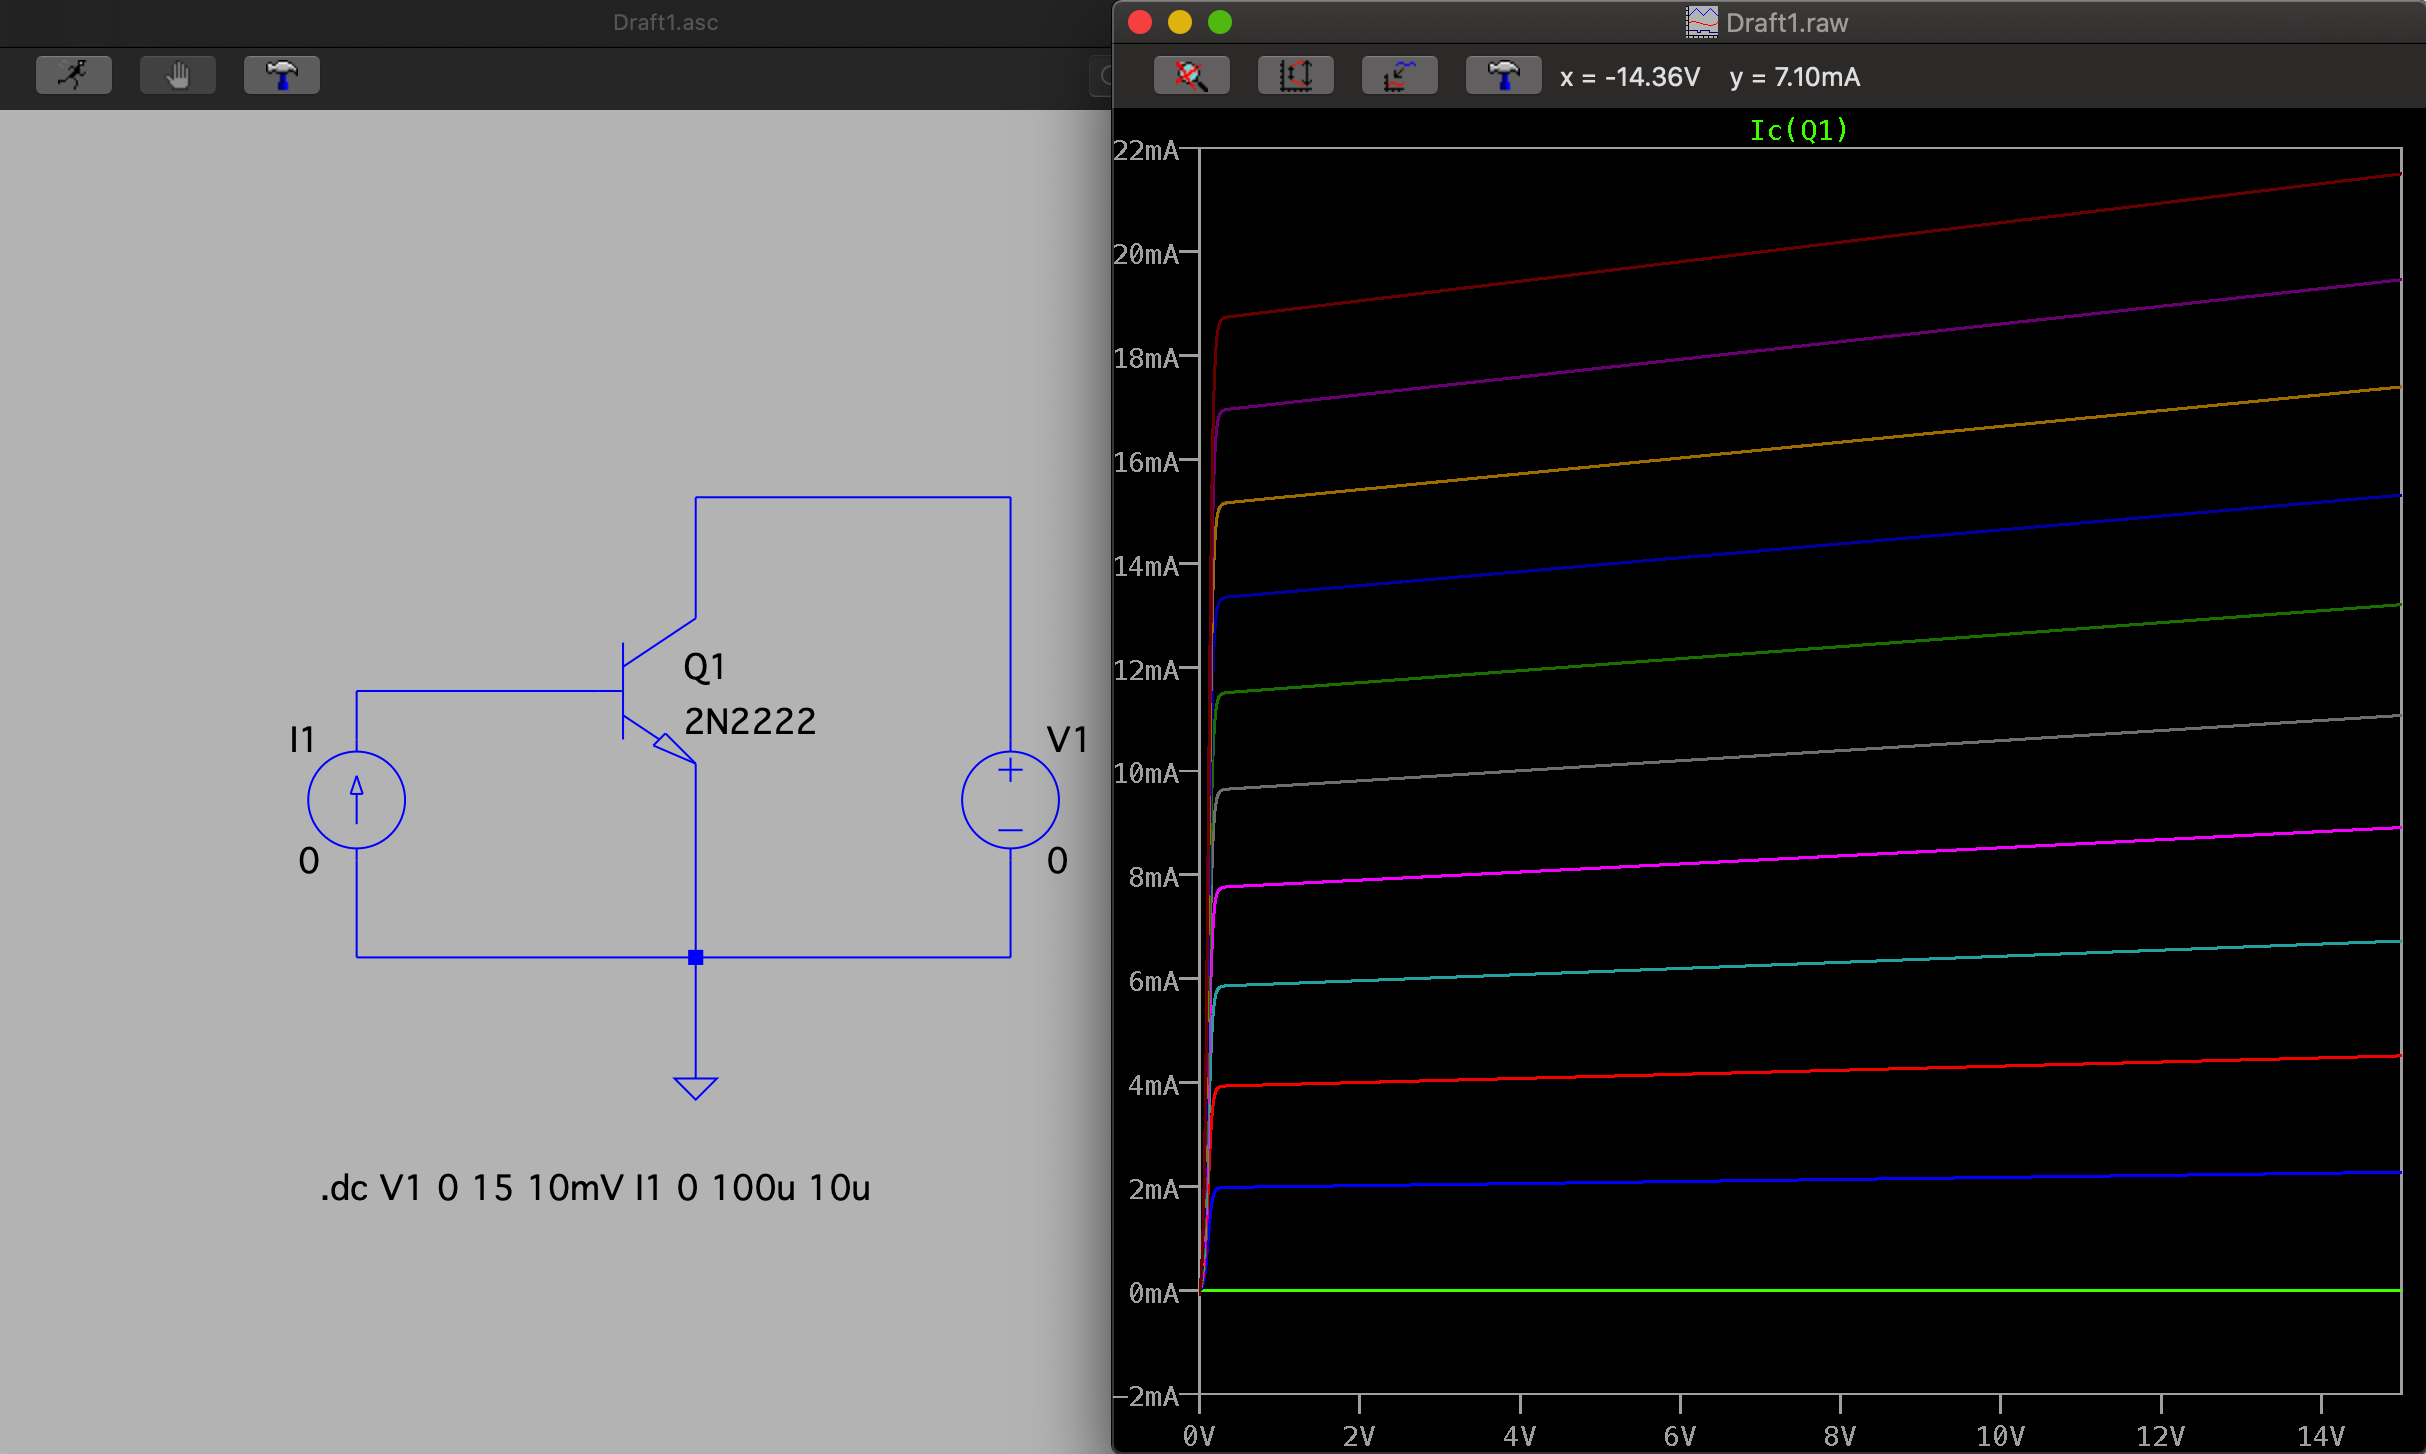
\includegraphics[width=\linewidth]{pictures/analysis_3.png}
        \end{minipage} 
        & 
        \begin{minipage}{.5\textwidth}
        \begin{itemize}
          \item Klickt auf 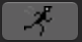
\includegraphics[scale=0.3]{pictures/run.png} (run) und LTspice startet die Simulation
        \item Wir wählen \textbf{IC(Q1)}, den Kollektorstrom.
        \end{itemize}
        \end{minipage} 
        \\
      \end{tabular}
    \end{table}
  \end{tiny} \end{spacing}
  
    \begin{spacing}{0.9} \begin{tiny}
      \begin{table}[h!]
        \begin{tabular}{p{10cm} }
          \hline
          \textbf{Ergebnis und Auswertung} \\
          \hline \\    
          Jeder Graph steht für einen simulierten Basisstrom. Per rechtem Mausklick $->$ View $->$ Steps könnt ihr einzelne Graphen zur
          detaillierten Analyse auswählen. \newline\newline Achtet darauf, welche Quelle ihr im $.dc ...$ simulation command zuerst wählt. \textbf{Quelle 1 ergibt im Diagramm die Abszisse, die Quelle 2 die Ordinate.}
        \end{tabular}
      \end{table}
    \end{tiny} \end{spacing}
    
     \end{frame}

     \begin{frame}[t]{NPN-Transistor}
      
      \begin{spacing}{0.6} \begin{tiny}
      
      Wenn ihr den Zusammenhang zwischen der Basisspannung $U_{be}$ und dem Kollektorstrom $I_c$ simulativ herausfinden wollt, müsst
      ihr die Schaltung leicht variieren. Dazu werden wir das schematic wie folgt anpassen. 

      \end{tiny} \end{spacing}
      \begin{spacing}{0.9} \begin{tiny}
      \begin{table}[h!]
        \begin{tabular}{p{3cm} p{7cm}}
          \hline
          \textbf{Erstellung des Schaltplans} & \\
          \hline \\
          \begin{minipage}{.3\textwidth}
            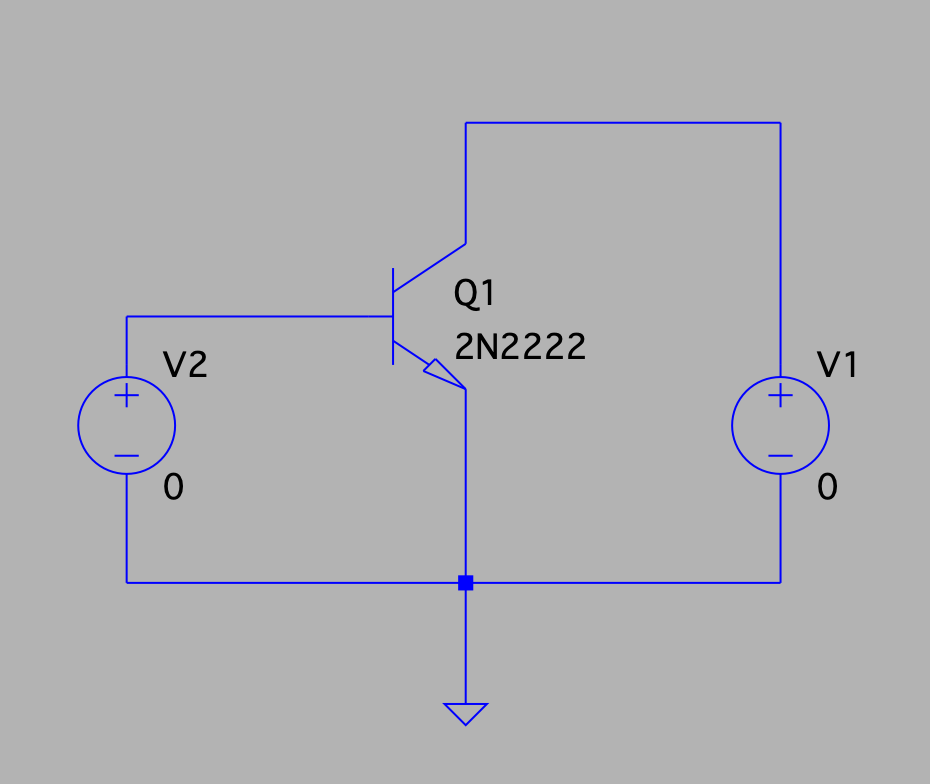
\includegraphics[width=\linewidth]{pictures/tran2.png}
          \end{minipage} 
          & 
          \begin{minipage}{.7\textwidth}
          \begin{itemize}
            \item Speichert das Projekt direkt als neue Datei ab (File $->$ save as ) 
            \item Löscht die Stromquelle (\textbf{F5}) und fügt eine Spannungsquelle hinzu. 
            \item Verdrahtet die Schaltung wieder vollstänndig (\textbf{F3})
            \item Super simple dieses mal :)
          \end{itemize}
          \end{minipage} 
          \\
           & \\
           \hline
           \textbf{Konfiguration der Simulation} & \\
           \hline \\
           \begin{minipage}{.3\textwidth}
            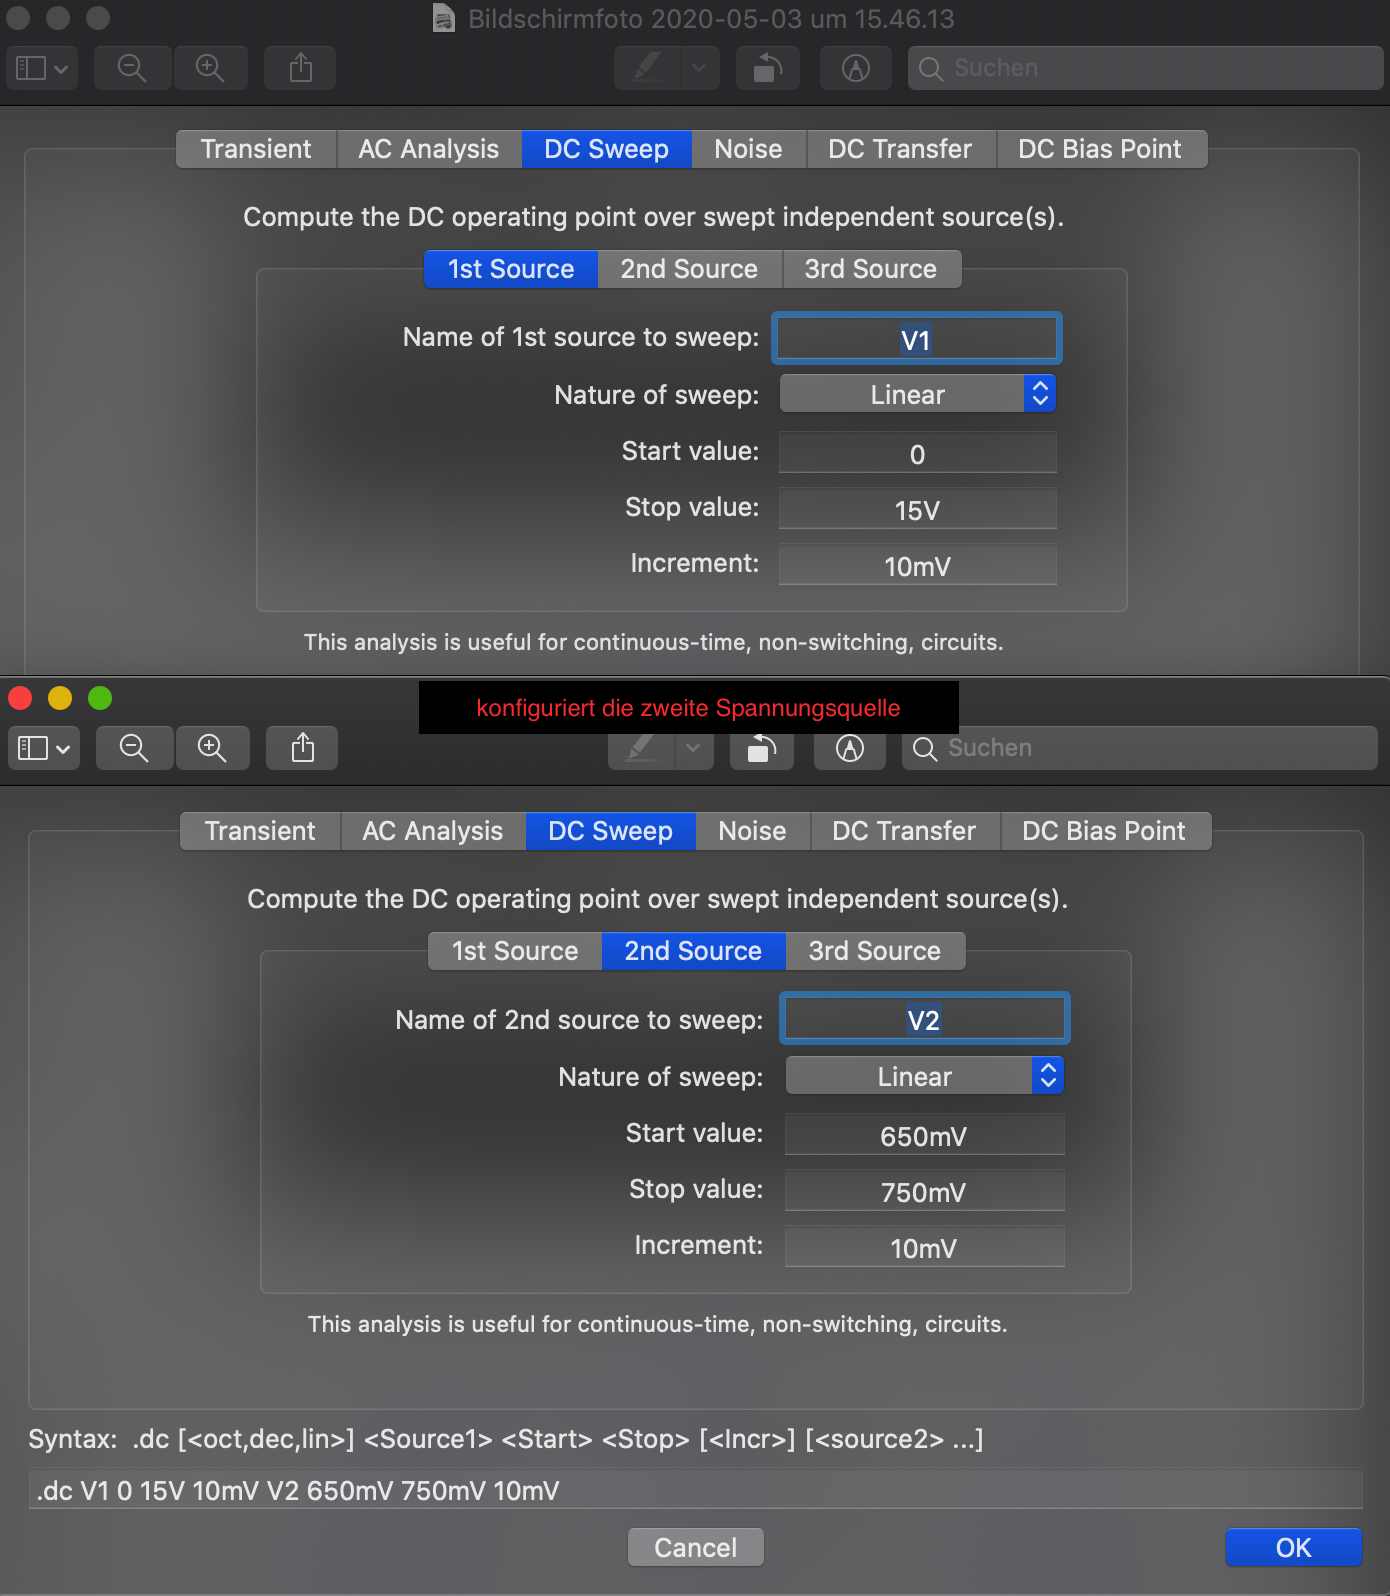
\includegraphics[width=0.8\linewidth]{pictures/simulationcmd_4.png}
          \end{minipage} 
          & 
          \begin{minipage}{.7\textwidth}
          \begin{itemize}
            \item Im Menu Simulation, wählt \textbf{Edit simulation command} und bliebt beim DC Sweep. 
            \item Unser Ziel ist es das Ausgangskennlinienfeld des 2N2222 simlativ zu bestimmen. Dazu verwenden wir dieses mal
            einen DC-Sweep mit einer Spannungsquelle, die die Basis-Emitterspannung $U_{be}$ simuliert und eine Spannungsquelle (V1) die die Spannung
            $U_{ce}$ simuliert. 
            \item V1 soll von 0 - 15V in 1V Schritten simuliert werden, V2 von 650 - 750 mV in 10mV Schritten.
            \item Bestätigt mit \textit{OK} und fügt die Simlationsansweisung dem schematic hinzu
          \end{itemize}
          \end{minipage} 
          \\
           & \\
           \hline
        \end{tabular}
      
      \end{table}
      
      \end{tiny} \end{spacing}
      
       \end{frame}



   \begin{frame}[t]{NPN-Transistor}
  
    \begin{spacing}{0.9} \begin{tiny}
    \begin{table}[h!]
      \begin{tabular}{p{5cm} p{5cm}}
        \hline
        \textbf{Simulation und Analyse} & \\
        \hline \\
        \begin{minipage}{.5\textwidth}
          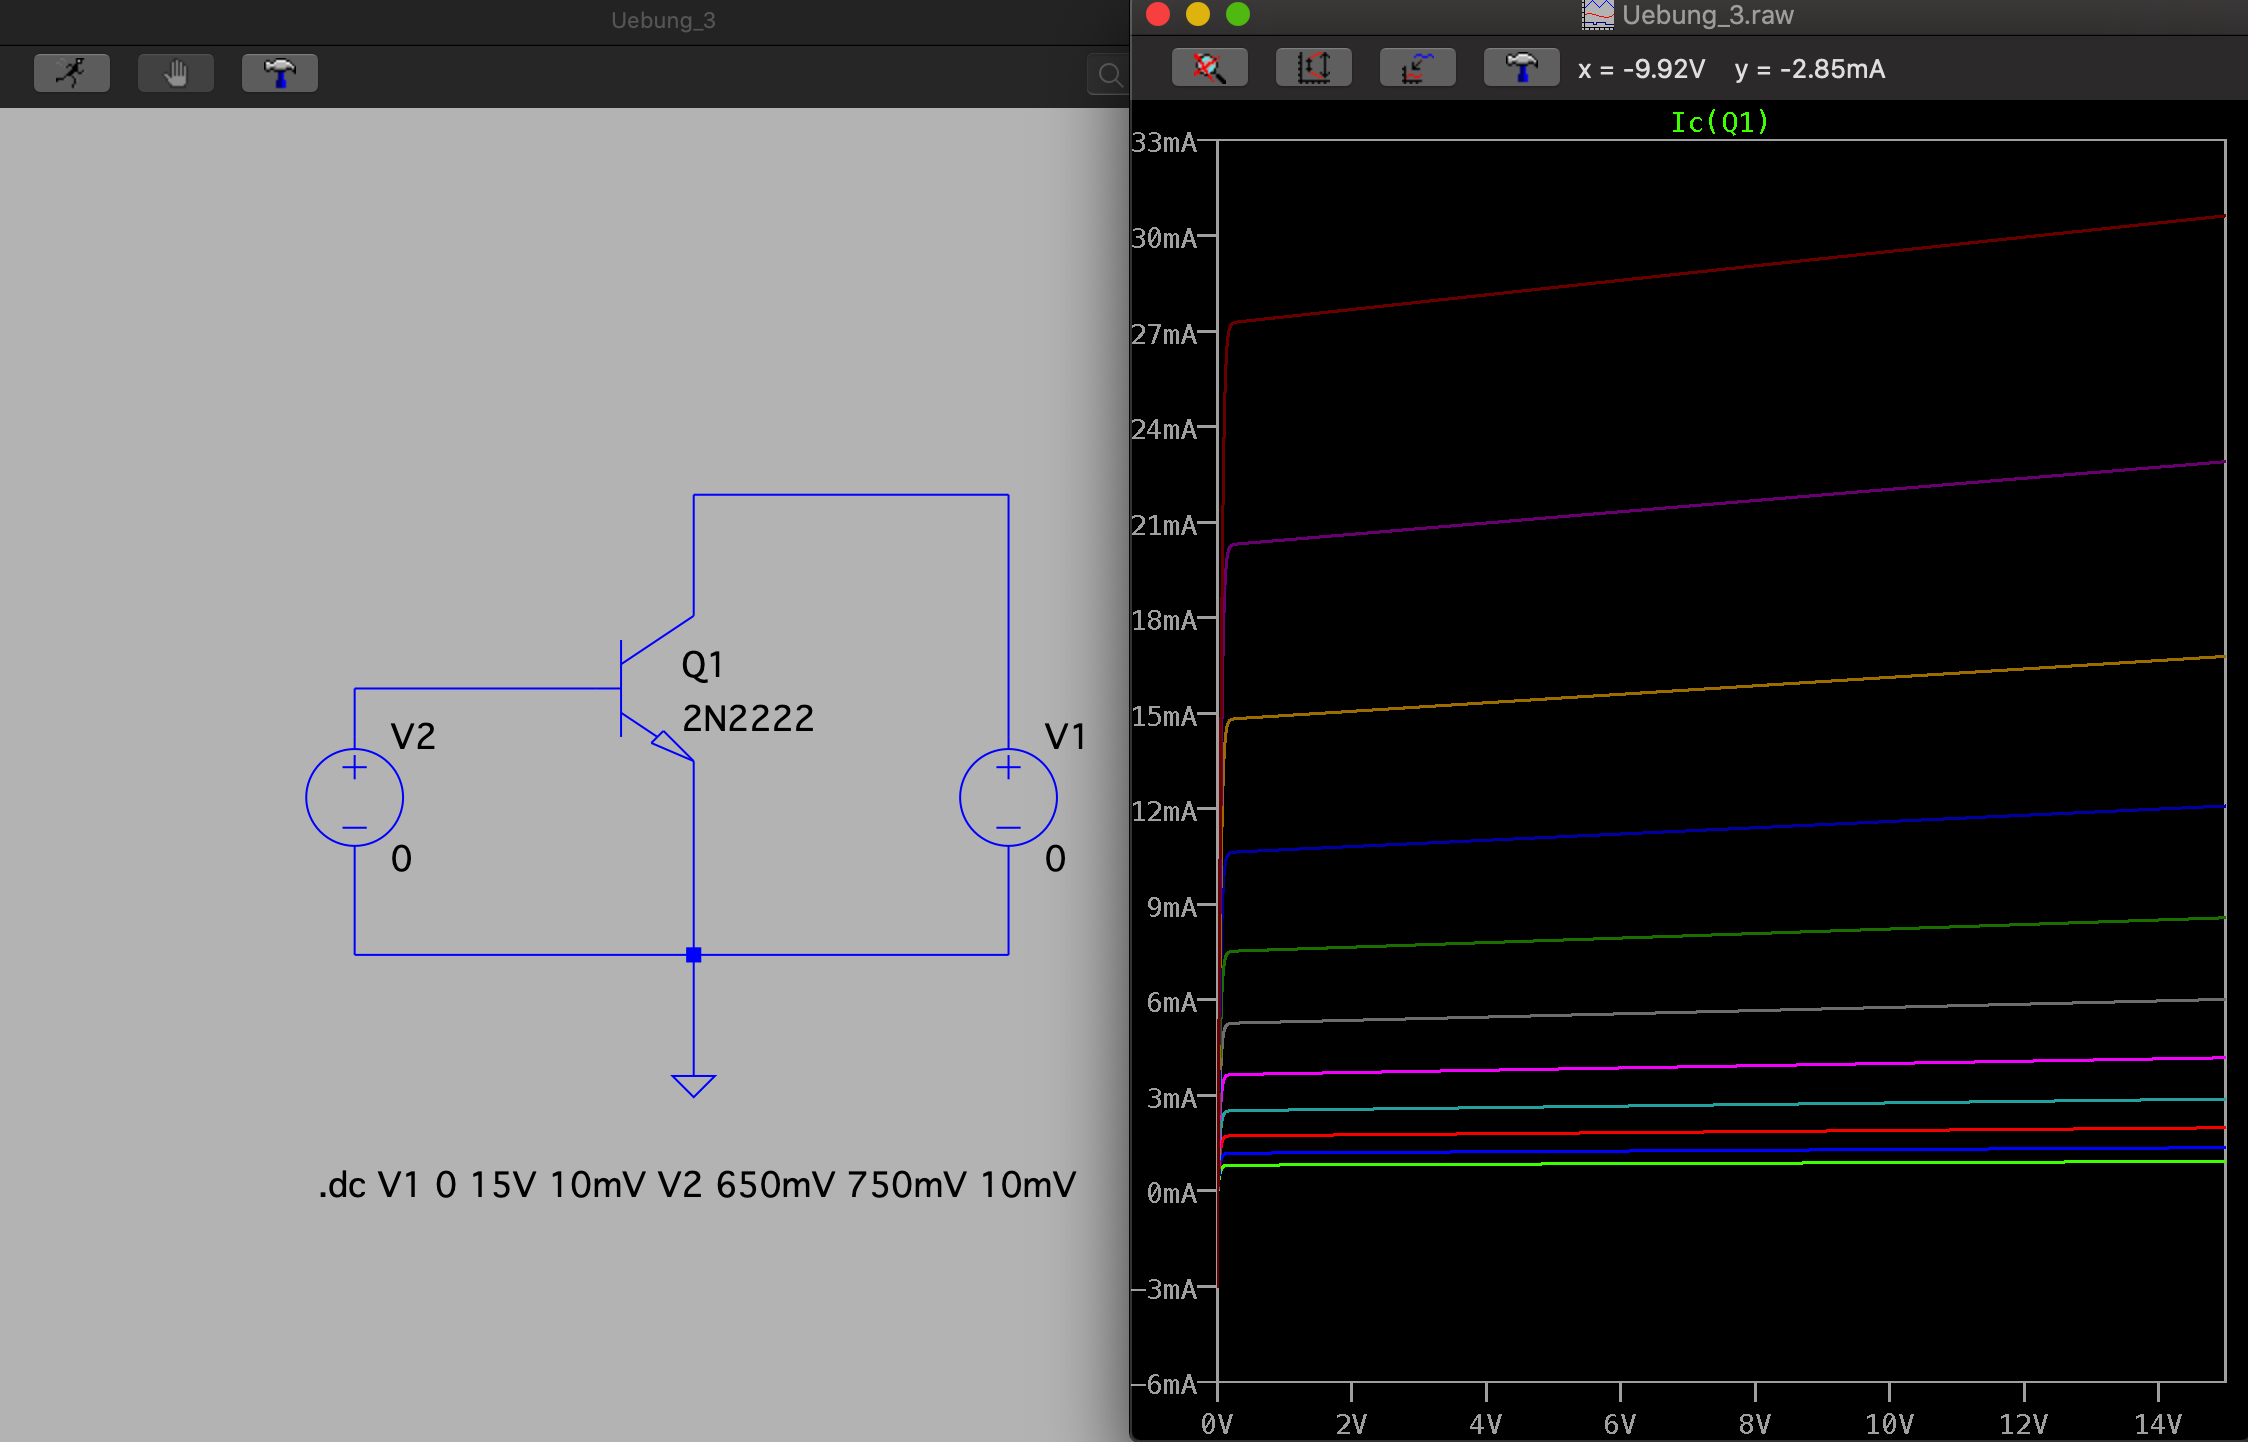
\includegraphics[width=\linewidth]{pictures/analysis_4.png}
        \end{minipage} 
        & 
        \begin{minipage}{.5\textwidth}
        \begin{itemize}
          \item Klickt auf 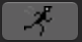
\includegraphics[scale=0.3]{pictures/run.png} (run) und LTspice startet die Simulation
        \item Wir wählen \textbf{IC(Q1)}, den Kollektorstrom.
        \end{itemize}
        \end{minipage} 
        \\
      \end{tabular}
    \end{table}
  \end{tiny} \end{spacing}
  
    \begin{spacing}{0.9} \begin{tiny}
      \begin{table}[h!]
        \begin{tabular}{p{10cm} }
          \hline
          \textbf{Ergebnis und Auswertung} \\
          \hline \\    
          Jeder Graph steht für eine simulierte $U_{be}$. Per rechtem Mausklick $->$ View $->$ Steps könnt ihr einzelne Graphen zur
          detaillierten Analyse auswählen. \newline\newline Achtet darauf, welche Quelle ihr im $.dc ...$ simulation command zuerst wählt. \textbf{Quelle 1 ergibt im Diagramm die Abszisse, die Quelle 2 die Ordinate.}
        \end{tabular}
      \end{table}
    \end{tiny} \end{spacing}
    
     \end{frame}